\chapter{环面几何}
\SourcePage{59}
我们将在域\footnote{可以把它看作特征为零的代数闭域，但环面几何对许多其他选择也适用，甚至可以在 $\ZZ$ 上开展。}$k$ 上工作。环面几何的基本口号是：
\begin{center}\Term{huanmianjihe}{环面几何}研究 $(\mathbb G_m)^n$ 的等变紧化。\end{center}
回忆 $\mathbb G_m=\Spec k[z,z^{-1}]$ 是代数几何中对应于 $\CC^\times$ 的对象。关键在于，包含关系 $(\mathbb G_m)^n\subset X$ 可用组合几何，即整格上的锥来描述。参考文献为 \cite{ref7,ref10,ref24}。
\section{幺半群与锥}
设 $M$ 是秩为 $d$ 的自由阿贝尔群，即 $M\simeq\ZZ^d$；记其对偶为 $N=\Hom_{\ZZ}(M,\ZZ)$。写作
\Eq{4.1}{M_{\QQ}=M\otimes_{\ZZ}\QQ=\Hom_{\ZZ}(N,\QQ),\qquad M_{\RR}=M\otimes_{\ZZ}\RR=M_{\QQ}\otimes_{\QQ}\RR.}
类似地，
\Eq{4.2}{N\subset N_{\QQ}\subset N_{\RR}.}
\thmnum{definition}{1}\begin{definition}\label{def:4.1}
设 $V$ 是 $\QQ$ 或 $\RR$ 上的向量空间。若 $0\in C\subset V$，且对标量域中每个 $\lambda>0$ 都有 $\lambda C\subset C$，则称 $C$ 为\Term{zhui}{锥}。若 $C+C\subset C$，则称 $C$ 为凸锥。
\end{definition}
\begin{Note}{4.1}若 $C$ 凸，则其在实向量空间 $V_{\RR}$ 中的闭包 $\overline C$ 是凸集；对闭锥而言，这一条件与 $C$ 为凸锥等价。\end{Note}
\thmnum{lemma}{1}\begin{lemma}\label{lem:4.1}
若 $C\subset M_{\RR}$ 是凸锥，则 $(C\cap M,+)$ 是饱和幺半群。其加法单位元为原点，而且它是交换的。
\end{lemma}
回忆，\Term{baoheyaobanqun}{饱和幺半群}的条件是：对每个 $m\in M$ 和每个正整数 $\lambda$，若 $\lambda m\in C\cap M$，则 $m\in C\cap M$。当锥不含非零线性子空间时，其可逆元群是平凡的。
\examnum{1}\begin{example}\label{ex:4.1}
取 $M=\ZZ$、$P=2\NN+3\NN$。有 $1\in M$、$2\in P$，但 $1\notin P$，所以 $P$ 不饱和。
\end{example}
\examnum{2}\begin{example}\label{ex:4.2}
考虑 $C=\RR_{\ge0}(0,1)+\RR_{\ge0}(k+1,-1)\subset\RR^2$，其中 $k$ 为非负整数。于是
\Eq{4.3}{C\cap M=\langle(0,1),(1,0),(k+1,-1)\rangle\simeq\NN^3/\bigl((0,k+1,0)\sim(1,0,1)\bigr).}
也就是说，唯一的生成关系为 $u+v=(k+1)w$。一般而言，若一个锥由 $d$ 个构成格基的向量 $m_1,\ldots,m_d$ 生成，即 $\det(m_1,\ldots,m_d)=\pm1$，则它的格点幺半群同构于 $\NN^d$。因此，所需结论可由以下两个行列式得到：
\Eq{4.4}{\det\begin{pmatrix}1&0\\0&1\end{pmatrix}=1,\qquad\det\begin{pmatrix}k+1&1\\-1&0\end{pmatrix}=1.}
\end{example}
\SourcePage{60}
\section{幺半群环}
\thmnum{definition}{2}\begin{definition}\label{def:4.2}
设 $S$ 为幺半群。与之关联的\Term{yaobanqunhuan}{幺半群环}为
\Eq{4.5}{k[S]=\left\{\sum_{m\in S}^{\text{有限}}a_m\chi^m:a_m\in k\right\},\qquad\chi^m\chi^{m'}=\chi^{m+m'}.}
\end{definition}
第一个问题是：何时 $k[S]$ 有限生成？$S$ 作为幺半群有限生成就是一个充分条件。
\examnum{3}\begin{example}\label{ex:4.3}
令 $C=\{0\}\cup(\RR_{\ge0}\times\RR_{>0})$。则 $S=C\cap M$ 不有限生成，因为对于所有 $a\in\NN$，格点 $(a,1)$ 都必须作为生成元。
\end{example}
\section{有理多面锥与 Gordan 引理}
\thmnum{definition}{3}\begin{definition}\label{def:4.3}
若存在 $m_1,\ldots,m_r\in M_{\QQ}$，使
\Eq{4.6}{C=\RR_{\ge0}m_1+\cdots+\RR_{\ge0}m_r,}
则称 $C\subset M_{\RR}$ 为\Term{youliduomianzhui}{有理多面锥}。
\end{definition}
注意，这意味着 $C\subset M_{\RR}$ 是闭的、凸的。
\thmnum{proposition}{2}\begin{proposition}[Gordan 引理]\label{prop:4.2}
若 $C\subset M_{\RR}$ 是有理多面锥，则 $C\cap M$ 有限生成。
\end{proposition}
这也说明 $k[C\cap M]$ 是有限生成 $k$ 代数。
\begin{proof}
把生成向量按正整数倍放大，可先令各 $m_i\in M$。由这些生成向量构成的集合
\Eq{4.7}{K=\left\{\sum_{i=1}^rt_im_i:0\le t_i\le1\right\}\subset M_{\RR}}
是紧的，因此 $K\cap M$ 有限。
\begin{custom}{断言 4.1}\hypertarget{claim:4.1}{}$K\cap M$ 生成 $C\cap M$。\end{custom}
对 $u=\sum r_im_i$，其中 $r_i\ge0$，把 $r_i$ 写成 $s_i+t_i$，其中 $s_i\in\NN$、$t_i\in[0,1)$。于是
\Eq{4.8}{u=\underbrace{\sum_i s_im_i}_{\text{由 }m_i\in K\cap M\text{ 生成}}+\underbrace{\sum_i t_im_i}_{\in K\cap M}.}
故结论成立。
\end{proof}
\Lecture{17}{2019年10月24日}
\section{凸几何中的若干事实}
现在列出一些定义与命题。设 $\sigma\subset N_{\RR}$ 为有理多面锥。
\begin{enumerate}[label=(\alph*)]
\item 对偶锥定义为
\Eq{4.9}{\sigma^\vee=\{u\in M_{\RR}:\text{对每个 }v\in\sigma,\ \langle u,v\rangle\ge0\}.}
\begin{custom}{事实 3}\hypertarget{fact:3}{}\begin{itemize}
\item 若 $\sigma$ 是多面锥，则 $\sigma^\vee$ 也是多面锥。
\item $\sigma=(\sigma^\vee)^\vee$。
\item $(\sigma_1\cap\sigma_2)^\vee=\sigma_1^\vee+\sigma_2^\vee$。
\end{itemize}\end{custom}
\SourcePage{61}
\item $\sigma+(-\sigma)=\RR\sigma\subset N_{\RR}$ 是 $\sigma$ 张成的线性子空间。定义 $\dim_{\RR}\sigma=\dim_{\RR}(\RR\sigma)$。
\item 若 $\sigma\cap(-\sigma)=\{0\}$，则称 $\sigma$ 为\Term{jianzhui}{尖锥}。
\begin{custom}{事实 4}\hypertarget{fact:4}{}下列条件等价：
\begin{enumerate}[label=(\roman*)]
\item $\sigma$ 为尖锥；\item $\dim\sigma^\vee=d$；\item 存在 $u\in\sigma^\vee$，使 $\sigma\cap u^\perp=\{0\}$。
\end{enumerate}\end{custom}
在环面几何中，$N_{\RR}$ 中的锥总是尖锥，而对应的 $M_{\RR}$ 中的锥总是 $d$ 维的。
\item 非尖锥的约化：令 $C=\sigma^\vee$、$L=C\cap(-C)=\sigma^\perp=(\RR\sigma)^\perp$。这是 $C$ 中最大的线性子空间。商空间 $M_{\RR}/L$ 中有尖锥 $\bar C$：它就是商映射 $q:M_{\RR}\to M_{\RR}/L$ 下的像 $q(C)$，而 $C=q^{-1}(\bar C)$。选择一个非典范分解 $M_{\RR}\simeq L\oplus M'_{\RR}$，便有 $M'_{\RR}\simeq M_{\RR}/L$；换言之，$C\simeq\bar C\times L$。
\item 锥 $\sigma\subset N_{\RR}$ 为多面锥，当且仅当它是有限个闭半空间的交。
\begin{proof}[证明概要]$\sigma^\vee=\sum_i\RR_{\ge0}u_i$ 等价于 $\sigma=\bigcap_iH_i$，其中 $H_i=(\RR_{\ge0}u_i)^\vee$。\end{proof}
\item 若 $u\ne0$ 且 $\sigma\subset(\RR_{\ge0}u)^\vee$，则称 $u^\perp\subset N_{\RR}$ 为支撑超平面。
\item 若 $u\in\sigma^\vee$，则 $u^\perp\cap\sigma$ 称为 $\sigma$ 的一个面 $\tau\subseteq\sigma$。
\begin{custom}{事实 5}\hypertarget{fact:5}{}\begin{itemize}
\item 每个面都是有理多面锥。
\item 在 $\RR\sigma\subset N_{\RR}$ 中，$\sigma$ 的相对拓扑边界是所有真面 $\tau\subsetneq\sigma$ 的并。
\item 若 $\tau_1,\tau_2\subseteq\sigma$ 为面，则 $\tau_1\cap\tau_2$ 也是面。
\item 若面 $\tau_1\subseteq\tau_2$ 满足 $\dim\tau_1=\dim\tau_2$，则 $\tau_1=\tau_2$。
\item 所有面中最小的维数为 $\dim_{\RR}(\sigma\cap(-\sigma))$。
\end{itemize}\end{custom}
\item 若 $\dim\tau=\dim\sigma-1$，则称面 $\tau$ 为侧面（余维一面）。
\begin{custom}{事实 6}\hypertarget{fact:6}{}\begin{itemize}
\item 每个面 $\tau\subseteq\sigma$ 都是若干侧面的交。
\item 每个余维二的面 $\omega\subseteq\sigma$，即 $\dim\omega=\dim\sigma-2$，恰好包含在两个侧面中。
\end{itemize}\end{custom}
\item 一维面称为极射线。若
\Eq{4.10}{\sigma=\RR_{\ge0}n_1+\cdots+\RR_{\ge0}n_r,}
则每条极射线都形如某个 $\RR_{\ge0}n_i$。在去除零向量和重复射线后，$r$ 最小当且仅当每个 $\RR_{\ge0}n_i$ 都是一条极射线。
\item 映射 $\tau\mapsto\tau^\perp\cap\sigma^\vee$ 给出 $\sigma$ 的面与 $\sigma^\vee$ 的面之间的双射；它反转包含关系，并使对应面的维数之和等于 $d$。
\end{enumerate}
\section{仿射环面簇}
固定域 $k$。
\thmnum{definition}{4}\begin{definition}\label{def:4.4}
$d$ 维\Term{huanmianzu}{仿射环面簇}是形如 $\Spec k[\sigma^\vee\cap M]$ 的概形，其中 $\sigma\subset N_{\RR}$ 为有理多面尖锥。
\end{definition}
注意，$k[M]$ 是 $k[\sigma^\vee\cap M]$ 的局部化，所以 $T_N=\Spec k[M]\subset\Spec k[\sigma^\vee\cap M]$ 是开嵌入。
\begin{Note}{4.2}Gordan 引理说明，这些仿射环面簇在 $k$ 上是有限型的。\end{Note}
\SourcePage{62}
\thmnum{proposition}{3}\begin{proposition}\label{prop:4.3}
若 $m_1,\ldots,m_s\in M$ 作为幺半群生成 $\sigma^\vee\cap M$，则理想
\Eq{4.11}{I=\ker(q:k[x_1,\ldots,x_s]\twoheadrightarrow k[\sigma^\vee\cap M]),\qquad q(x_1^{a_1}\cdots x_s^{a_s})=\chi^{a_1m_1+\cdots+a_sm_s}}
由下列二项式生成：
\Eq{4.12}{G=\left\{x_1^{a_1}\cdots x_s^{a_s}-x_1^{b_1}\cdots x_s^{b_s}:\sum_i a_im_i=\sum_i b_im_i,\ a_i,b_i\in\NN\right\}.}
\end{proposition}
\begin{proof}
映射 $q$ 在如下分次下是齐次的：
\Eq{4.13}{\deg x_i=m_i,\qquad\deg\chi^m=m.}
因此 $I$ 是 $M$ 分次齐次理想，从而由 $M$ 分次齐次多项式生成。对齐次多项式 $f=\sum_A\alpha_Ax^A\in I$，各非零项都满足
\Eq{4.14}{\sum_i A_im_i=m,\qquad q(f)=\left(\sum_A\alpha_A\right)\chi^m.}
所以 $f\in I$ 当且仅当 $\sum_A\alpha_A=0$。利用 $x^A-x^{A'}\in G\subset I$，把 $x^A$ 换成 $x^{A'}$，并对非零项数作递减归纳即可。
\end{proof}
\begin{Note}{4.3}由 $G$ 中这类元素生成的理想称为环面理想。\end{Note}
\section{\texorpdfstring{$k$}{k}有理点}
回忆，对概形 $X$ 和域 $K$，可以考虑 $K$ 值点的集合（即概形论意义下的点）。在 $X$ 是 $k$ 概形且 $K/k$ 为域扩张时，
\Eq{4.15}{X(K)=\Hom_k(\Spec K,X)=\{(x,\iota):x\in X,\ \iota:\kappa(x)\hookrightarrow K\text{ 为 }k\text{ 嵌入}\},}
其中 $\kappa(x)=\OO_{X,x}/\mathfrak m_x$ 为剩余域。当 $K=k$ 时，这就是剩余域为 $k$ 的有理点；在代数闭域上的有限型情形，也就是极大谱 $\mathrm{m\text{-}Spec}$。
\begin{Note}{4.4}若 $k$ 代数闭且 $X/k$ 有限型，则 $X(k)$ 就是闭点的集合。\end{Note}
\thmnum{proposition}{4}\begin{proposition}\label{prop:4.4}
若 $X=\Spec k[\sigma^\vee\cap M]$，则
\Eq{4.16}{X(k)=\Hom_{\Mon}(\sigma^\vee\cap M,(k,\cdot)).}
\end{proposition}
注意，右侧使用的是乘法幺半群 $(k,\cdot)$。
\begin{proof}
我们知道
\Eq{4.17}{X(k)=\Hom_{k\text{-}\mathrm{Alg}}(k[\sigma^\vee\cap M],k),}
在代数闭情形下也等于该环的极大谱；这里把 $k$ 看作环。把代数同态 $\Phi$ 限制到单项式，并令 $\varphi(m)=\Phi(\chi^m)$，便得到
\Eq{4.18}{\Hom_{\Mon}(\sigma^\vee\cap M,(k,\cdot)).}
\end{proof}
\examnum{4}\begin{example}\label{ex:4.4}
取 $C=M_{\RR}$，考虑 $\Hom_{\Mon}(M,(k,\cdot))$。$M$ 中每个元素都可逆，所以这等于 $\Hom_{\Mon}(M,k^\times)=N\otimes_{\ZZ} k^\times\simeq(k^\times)^d$。
\end{example}
\examnum{5}\begin{example}\label{ex:4.5}
令 $C=\RR_{\ge0}^2$。则
\Eq{4.19}{k[\sigma^\vee\cap M]=k[x,y],}
其中 $x=\chi^{(1,0)}$、$y=\chi^{(0,1)}$。每个 $\varphi$ 由 $x\mapsto\lambda$、$y\mapsto\mu$ 确定。因此
\Eq{4.20}{\Hom_{\Mon}(\sigma^\vee\cap M,(k,\cdot))=k^2.}
\end{example}
\SourcePage{63}
设 $X=\Spec\CC[\sigma^\vee\cap M]$。事实上，存在一种“矩映射”
\Eq{4.21}{X(\CC)\longrightarrow\sigma^\vee.}
位于 $\sigma^\vee$ 的一个 $k$ 维面的相对内部的点 $p$，其纤维同胚于 $(S^1)^k$。
\examnum{6}\begin{example}\label{ex:4.6}
考虑 $\CC^2\to\RR_{\ge0}^2$，$(\lambda,\mu)\mapsto(|\lambda|,|\mu|)$。
\end{example}
\section{环面开子概形}
回忆，若 $f\in R$，则 $D_f=\Spec R_f\subset\Spec R$ 是一个基本开集。
\thmnum{proposition}{5}\begin{proposition}\label{prop:4.5}
设 $\sigma\subset N_{\RR}$ 为有理多面锥，$\tau\subseteq\sigma$ 为面。则 $\sigma^\vee\hookrightarrow\tau^\vee$ 定义同态
\Eq{4.22}{k[\sigma^\vee\cap M]\hookrightarrow k[\tau^\vee\cap M].}
这个同态就是在一个元素处局部化。特别地，
\Eq{4.23}{U_\tau:=\Spec k[\tau^\vee\cap M]\hookrightarrow\Spec k[\sigma^\vee\cap M]=:U_\sigma=X}
是一个基本开子概形。
\end{proposition}
\begin{proof}
写 $\tau=\sigma\cap m^\perp$，其中 $m\in\sigma^\vee\cap M$。于是 $m$ 在 $\sigma\setminus\tau$ 上严格为正。我们断言
\Eq{4.24}{\tau^\vee\cap M=(\sigma^\vee\cap M)+\NN(-m).}
包含关系 $\supseteq$ 显然成立。反之，取 $u\in\tau^\vee\cap M$，要证明当 $\lambda\gg0$ 时，$u+\lambda m\in\sigma^\vee$。写 $\sigma=\RR_{\ge0}n_1+\cdots+\RR_{\ge0}n_s$。我们需要对所有 $i$ 有
$\langle u+\lambda m,n_i\rangle=\langle u,n_i\rangle+\lambda\langle m,n_i\rangle\ge0$。
若 $n_i\in\tau$，则第二项为零而第一项非负；若 $n_i\notin\tau$，则第二项的系数严格为正，所以当 $\lambda\gg0$ 时整个表达式为正。因此每个 $u\in\tau^\vee\cap M$ 都满足所需条件，从而
$k[\tau^\vee\cap M]=k[\sigma^\vee\cap M]_{\chi^m}\subset k[M]$。
\end{proof}
\Lecture{18}{2019年10月29日}
\thmnum{definition}{5}\begin{definition}\label{def:4.5}
称 $U_\tau=\Spec k[\tau^\vee\cap M]\subset X$ 为基本开集。
\end{definition}
\examnum{7}\begin{example}\label{ex:4.7}
设 $\sigma=\RR_{\ge0}^2\subset N_{\RR}=\RR^2$。记竖直面为 $\tau_1$，水平面为 $\tau_2$，原点面为 $0$。则 $\tau_1^\vee$ 是上半平面，$\tau_2^\vee$ 是右半平面，而 $0^\vee$ 是整个平面。因此
\Eq{4.25}{U_{\tau_1}=\Spec k[x,y]_x=\mathbb G_m\times\mathbb A^1,}
\Eq{4.26}{U_{\tau_2}=\Spec k[x,y]_y=\mathbb A^1\times\mathbb G_m,}
\Eq{4.27}{U_0=\Spec k[x,y]_{xy}=\mathbb G_m^2.}
\end{example}
\section{有理函数、维数与正规性}
\thmnum{proposition}{6}\begin{proposition}\label{prop:4.6}
考虑有理多面锥 $C\subset M_{\RR}$，记
\Eq{4.28}{L=\RR C=C+(-C).}
则：
\begin{enumerate}[label=(\alph*)]
\item \Eq{4.29}{\Quot k[C\cap M]=\Quot k[L\cap M]=k(L\cap M).}
\item 每个仿射环面簇都是正规的。
\SourcePage{64}
\item $\dim\Spec k[C\cap M]=\dim_{\RR} L$。
\end{enumerate}
\end{proposition}
\begin{proof}
(a) 显然成立。(b) 把 $C=v_1^\vee\cap\cdots\cap v_r^\vee$ 写成半空间的交，有
\Eq{4.30}{C\cap M=\bigcap_{i=1}^r(M\cap v_i^\vee),}
因而
\Eq{4.31}{k[C\cap M]=\bigcap_i k[M\cap v_i^\vee]\subset k[M].}
在共同分式域中，整闭环的交仍整闭。而每个半空间对应的环，在选取合适的格基后，都形如
\Eq{4.32}{k[M\cap v_i^\vee]\simeq k[x_1^{\pm1},\ldots,x_{d-1}^{\pm1},x_d],}
这是多项式环的局部化，因此正规，结论得证。(c) $\Spec k[C\cap M]$ 含有开稠密子概形 $\Spec k[L\cap M]\simeq\mathbb G_m^{\dim_{\RR} L}$。
\end{proof}
\section{环面分层}
这些分层就是 $\mathbb G_m^d$ 轨道的闭包。
\thmnum{lemma}{7}\begin{lemma}\label{lem:4.7}
设 $\sigma\subset N_{\RR}$ 为有理多面尖锥，$\dim N_{\RR}=d$。取面 $\tau\subseteq\sigma$，令 $L=\RR\tau=\tau+(-\tau)$ 为其线性张成空间。则
\Eq{4.33}{\tau^\perp\cap\sigma^\vee=L^\perp\cap\sigma^\vee}
是商空间 $N_{\RR}/L$ 中的锥 $\sigma/L$ 的对偶锥；$\sigma$ 在该商空间中的像 $\sigma/L$ 仍为尖锥。
\end{lemma}
因此有 $\sigma\twoheadrightarrow\sigma/L$，且 $(\sigma/L)^\vee=\tau^\perp\cap\sigma^\vee$。对偶化得到环同态
\Eq{4.34}{k[(\tau^\perp\cap\sigma^\vee)\cap M]\hookrightarrow k[\sigma^\vee\cap M],}
它诱导一个占优\footnote{即像是稠密的。}态射
\Eq{4.35}{\underbrace{\Spec k[\sigma^\vee\cap M]}_{X=U_\sigma}\xrightarrow{\pi}\underbrace{\Spec k[(\tau^\perp\cap\sigma^\vee)\cap M]}_{U_{\sigma/L}}.}
这个映射可如下理解：有理子空间 $L\subset N_{\RR}$ 给出 $M_{\RR}\twoheadrightarrow M_{\RR}/L^\perp$，从而得到子环面
\Eq{4.36}{T_L=\Spec k[M/(L^\perp\cap M)]\subset T=\mathbb G_m^d.}
这个环面作用在上述映射的纤维上。事实上，$\pi$ 就是 $X$ 关于 $T_L$ 的范畴商。\footnote{关键是取轨道的闭包，从而至少得到一个 Hausdorff 空间。}
现在要构造截面 $\iota:U_{\sigma/L}\to U_\sigma$。我们知道 $\tau^\perp\cap\sigma^\vee$ 是 $\sigma^\vee$ 的一个面。定义理想
\Eq{4.37}{I_\tau=(\chi^m)_{m\in(\sigma^\vee\cap M)\setminus\tau^\perp}\subset k[\sigma^\vee\cap M].}
取此理想的商便定义了 $\iota^*$。我们要验证复合 $\pi\circ\iota$ 是 $U_{\sigma/L}$ 上的恒等映射。回忆有
\Eq{4.38}{k[(\tau^\perp\cap\sigma^\vee)\cap M]\xrightarrow{\pi^*}k[\sigma^\vee\cap M]\xrightarrow{\iota^*}k[\sigma^\vee\cap M]/I_\tau.}
\SourcePage{65}
此复合在两侧由单项式 $(\tau^\perp\cap\sigma^\vee)\cap M$ 给出的 $k$ 向量空间基之间诱导显然的双射。因此 $\pi\circ\iota=\id$。
\begin{Note}{4.5}注意，$k[(\tau^\perp\cap\sigma^\vee)\cap M]=k[\sigma^\vee\cap M]^{T_L}$；对 $m\in\sigma^\vee\cap M$，其 $T_L$ 权为 $\deg_{T_L}\chi^m=q(m)$，其中 $q:M\to M/(L^\perp\cap M)$。\end{Note}
\thmnum{definition}{6}\begin{definition}\label{def:4.6}
形如 $U_{\sigma/L}\subset U_\sigma$ 的闭子概形称为\Term{huanmianfenceng}{环面分层}。特别地，取 $\tau=\{0\}$ 时，整个环面簇自身也是一个分层。
\end{definition}
\examnum{8}\begin{example}\label{ex:4.8}
取 $\tau=\RR_{\ge0}\times\{0\}\subset\RR_{\ge0}^2=\sigma$。$\tau^\perp\cap\sigma^\vee$ 是 $\sigma^\vee$ 内的竖直半射线。把 $\sigma^\vee$ 的生成元记为 $x,y$，则
\Eq{4.39}{k[(\tau^\perp\cap\sigma^\vee)\cap M]=k[y]\hookrightarrow k[x,y],}
对应的映射 $\mathbb A^2\to\mathbb A^1$ 为 $(x,y)\mapsto y$。此时 $U_{\sigma/L}=Z(x)$，即 $y$ 轴。
\end{example}
\examnum{9}\begin{example}\label{ex:4.9}
令
\Eq{4.40}{\sigma^\vee=\RR_{\ge0}(1,0,0)+\RR_{\ge0}(1,1,0)+\RR_{\ge0}(1,1,1)+\RR_{\ge0}(1,0,1)\subset\RR^3.}
分别把生成元记为 $x,z,y,w$。于是
\Eq{4.41}{k[\sigma^\vee\cap M]=k[x,y,z,w]/(xy-zw),}
因为 $xy$ 和 $zw$ 都等于 $\chi^{(2,1,1)}$。有
\Eq{4.42}{\sigma^\vee\cap\tau^\perp=\RR_{\ge0}(1,0,0)+\RR_{\ge0}(1,1,0),}
这对应于 $\sigma$ 的极射线 $\tau$。因此
\Eq{4.43}{k[(\sigma^\vee\cap\tau^\perp)\cap M]\simeq k[x,z],}
而 $I_\tau=(w,y)$。具体地，
\Eq{4.44}{\pi^*:k[x,z]\longrightarrow k[x,y,z,w]/(xy-zw),}
\Eq{4.45}{\iota^*:k[x,y,z,w]/(xy-zw)\xrightarrow{/\,(w,y)}k[x,z].}
\end{example}
\section{整体化：扇}
\thmnum{definition}{7}\begin{definition}\label{def:4.7}
$N_{\RR}$ 中的\Term{shan}{扇}是有理多面尖锥 $\sigma\subset N_{\RR}$ 的非空集合 $\Sigma$，满足：
\begin{enumerate}[label=(\roman*)]
\item 对每个 $\sigma\in\Sigma$，其每个面 $\tau\subseteq\sigma$ 也属于 $\Sigma$；
\item 对每个 $\sigma,\sigma'\in\Sigma$，$\sigma\cap\sigma'$ 是二者的共同面。
\end{enumerate}
扇的支撑为
\Eq{4.46}{|\Sigma|=\bigcup_{\sigma\in\Sigma}\sigma.}
若 $|\Sigma|=N_{\RR}$，则称 $\Sigma$ 完备。
\end{definition}
稍后将看到，扇的完备性等价于相应环面簇的固有性。
\examnum{10}\begin{example}[（$\PP^2$）]\label{ex:4.10}
考虑图~\ref{fig:4.1} 中的三个锥。$\sigma_0$ 由 $(1,0),(0,1)$ 张成，$\sigma_1$ 由 $(0,1),(-1,-1)$ 张成，$\sigma_2$ 由 $(1,0),(-1,-1)$ 张成。记 $(0,1)$、$(1,0)$、$(-1,-1)$ 所生成的射线分别为 $\tau_1,\tau_2,\tau_3$。这些 $\sigma_i$、$\tau_i$ 以及原点共同构成一个扇。
\end{example}
\SourcePage{66}
\OriginalFigure{fig-4-1.pdf}{0.6027}{$\RR^2$ 中对应于 $\PP^2$ 的扇。}{fig:4.1}
\examnum{11}\begin{example}\label{ex:4.11}
沿用例题~\ref{ex:4.10} 的记号。只取右上象限 $\RR_{\ge0}^2$ 以及由 $(-1,-1)$ 张成的射线，得到扇
\[\{\sigma_0,\tau_1,\tau_2,\tau_3,0\}.\]
\end{example}
\examnum{12}\begin{example}\label{ex:4.12}
当 $d=1$ 时，$\Sigma$ 为以下三种扇之一：
\Eq{4.47}{\Sigma=\{\bullet\},\qquad\vcenter{\hbox{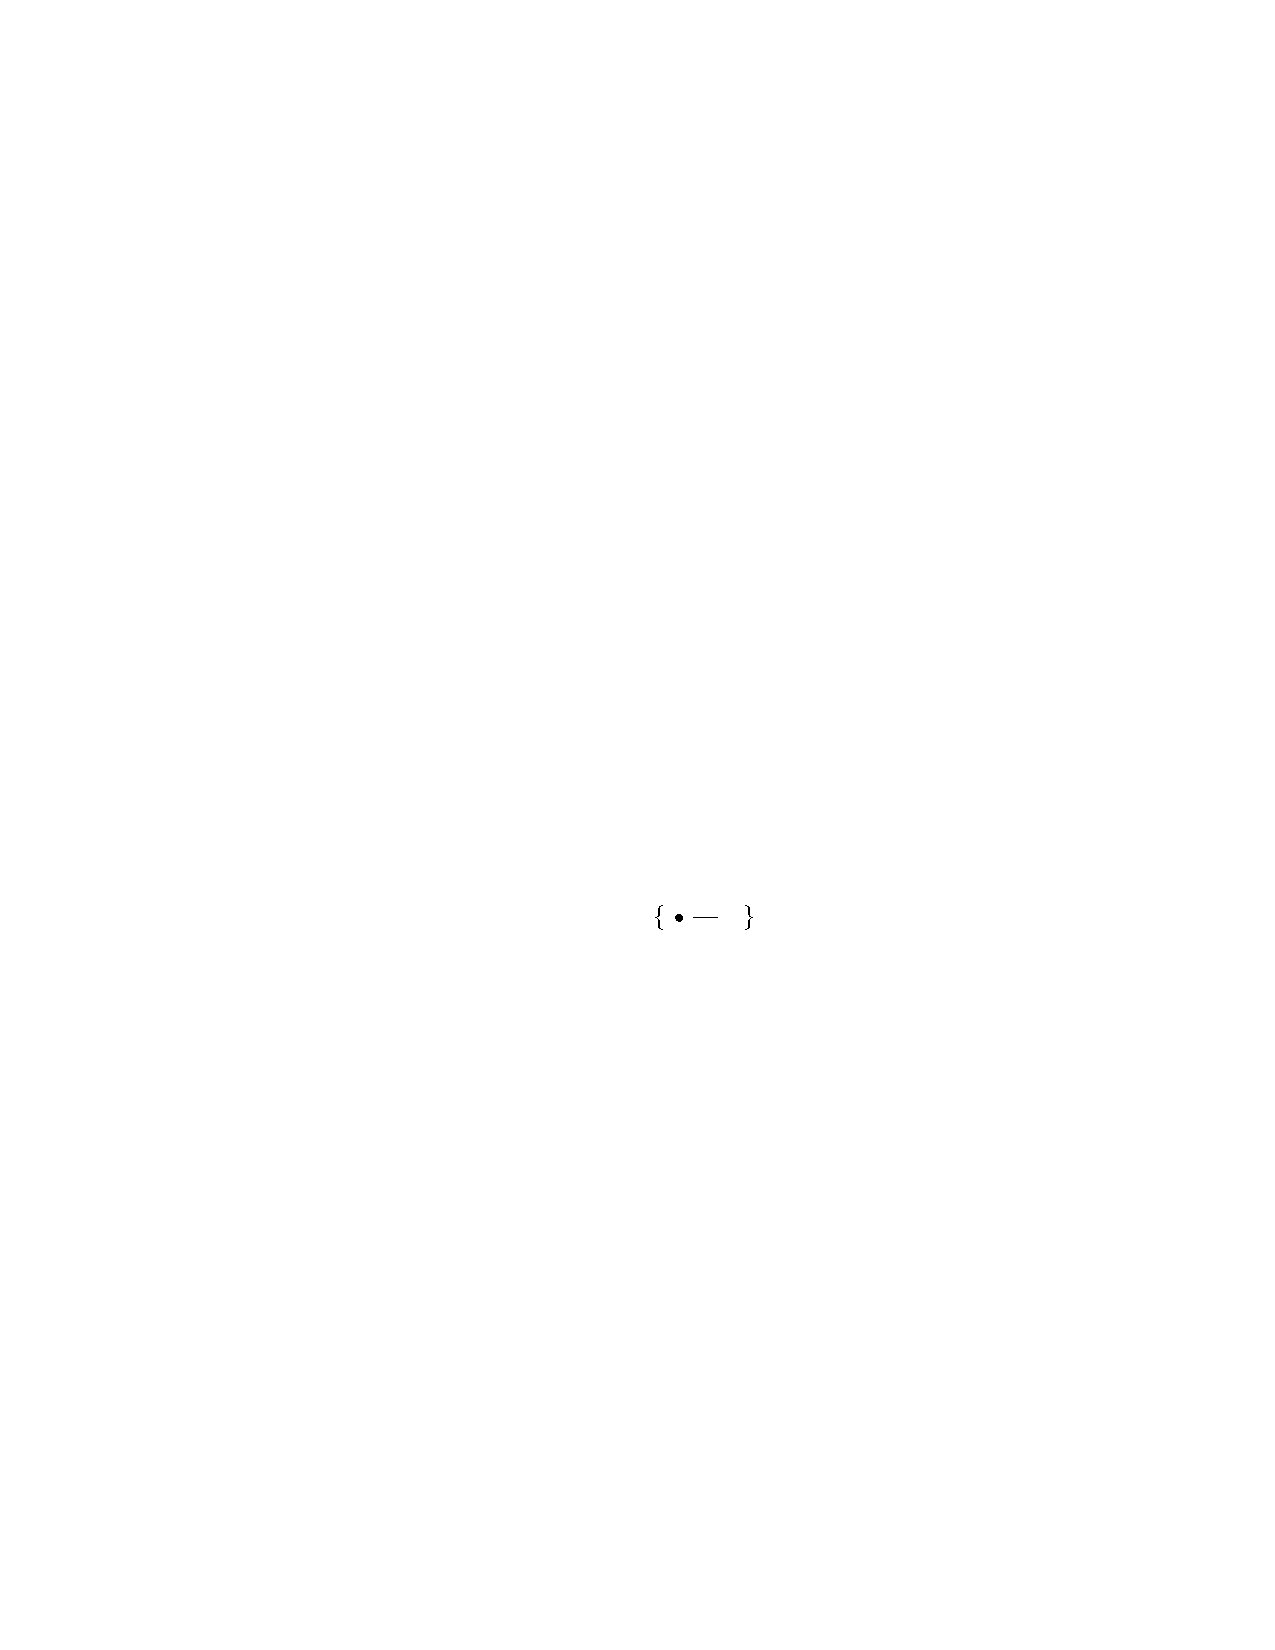
\includegraphics[width=0.1313\linewidth]{images/diagram-4-47a.pdf}}},\qquad\vcenter{\hbox{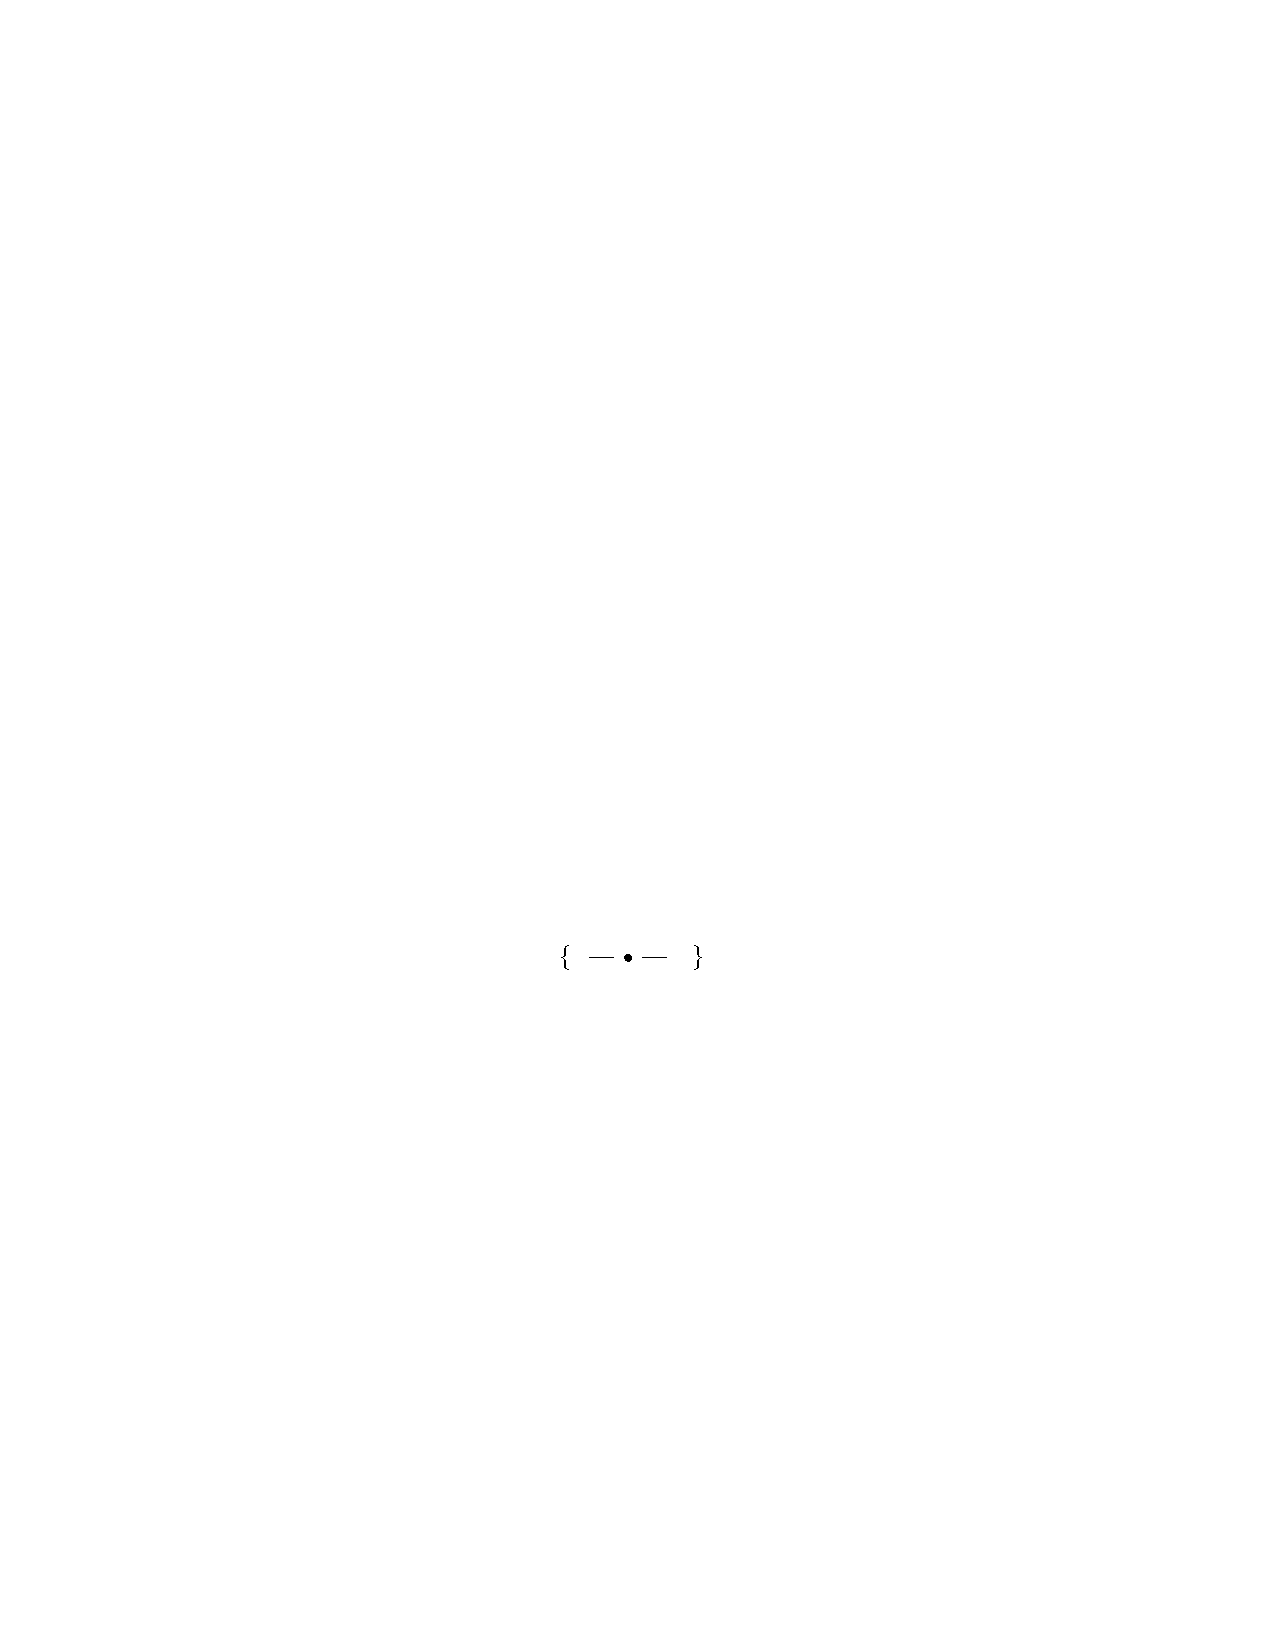
\includegraphics[width=0.1818\linewidth]{images/diagram-4-47b.pdf}}}.}
\end{example}
现在构造关联的概形。给定扇 $\Sigma$，对其中每个锥 $\sigma$，取仿射环面簇 $U_\sigma\supset\mathbb G_m^d$。对 $\sigma,\sigma'\in\Sigma$，不妨只考虑极大锥，其交是各自的面，所以有开嵌入
\Eq{4.48}{\begin{tikzcd}\&U_\sigma\\U_{\sigma\cap\sigma'}\arrow[ur,hook]\arrow[dr,hook]\&\\\&U_{\sigma'}.\end{tikzcd}}
于是
\Eq{4.49}{X(\Sigma)=\varinjlim_{\sigma\in\Sigma}U_\sigma}
是一个概形。我们将对 $\PP^2$ 显式检查这种相容性。
\section{例题：\texorpdfstring{$\PP^2$}{P²}}
设 $\Sigma$ 如例题~\ref{ex:4.10} 所示。对偶化得到图~\ref{fig:4.2} 中的锥。
\SourcePage{67}
\OriginalFigure{fig-4-2.pdf}{0.6498}{例题~\ref{ex:4.10} 中的扇所对应的对偶锥。}{fig:4.2}
这些锥给出如下开集：
\Eq{4.50}{U_{\sigma_0}=\Spec k[\underbrace{\chi^{(1,0)}}_{u_0},\underbrace{\chi^{(0,1)}}_{u_1}],}
\Eq{4.51}{U_{\sigma_1}=\Spec k[\underbrace{\chi^{(-1,1)}}_{v_0},\underbrace{\chi^{(-1,0)}}_{v_1}],}
\Eq{4.52}{U_{\sigma_2}=\Spec k[\underbrace{\chi^{(0,-1)}}_{w_0},\underbrace{\chi^{(1,-1)}}_{w_1}].}
现在把这些坐标图粘合起来。$\sigma_0\cap\sigma_1$ 是正 $y$ 轴，其对偶锥 $\sigma_0^\vee+\sigma_1^\vee$ 是上半平面，对应于
\Eq{4.53}{k[u_0,u_1]_{u_0}=k[v_0,v_1]_{v_1}.}
开嵌入 $U_{\sigma_0\cap\sigma_1}\hookrightarrow U_{\sigma_0}$ 对应于
\Eq{4.54}{k[u_0,u_1]\hookrightarrow k[u_0,u_1]_{u_0},}
而 $U_{\sigma_0\cap\sigma_1}\hookrightarrow U_{\sigma_1}$ 对应于
\Eq{4.55}{k[v_0,v_1]\hookrightarrow k[v_0,v_1]_{v_1}.}
二者确实一致。具体的坐标变换为
\Eq{4.56}{v_0=u_0^{-1}u_1,\qquad v_1=u_0^{-1}.}
因此得到
\Eq{4.57}{X(\Sigma)\simeq\PP^2=\operatorname{Proj}k[x_0,x_1,x_2],}
\SourcePage{68}
其中具体地，
\Eq{4.58}{u_0=x_1/x_0,\qquad u_1=x_2/x_0,}
\Eq{4.59}{v_0=u_0^{-1}u_1=(x_0/x_1)(x_2/x_0)=x_2/x_1,\qquad v_1=u_0^{-1}=x_0/x_1,}
\Eq{4.60}{w_0=u_1^{-1}=x_0/x_2,\qquad w_1=x_1/x_2.}
\section{作为环面簇的\texorpdfstring{$\PP_k^d$}{Pᵈ}}
对 $i\in\{1,\ldots,d\}$，记
\Eq{4.61}{v_i=e_i=(0,\ldots,0,1,0,\ldots,0)\in\RR^d,}
并令
\Eq{4.62}{v_0=-\sum_{i=1}^de_i=(-1,\ldots,-1).}
令 $\Sigma$ 为射线为 $\RR_{\ge0}v_i$ 的完备扇。
\Lecture{19}{2019年10月31日}
\section{环面分层}
设 $\Sigma$ 为扇，$\tau\in\Sigma$。它给出相应子环面的不动点闭子集。具体地，令 $N_\tau=N\cap\RR\tau$，$M_\tau=\Hom(N_\tau,\ZZ)$，$T_\tau=\Spec k[M_\tau]$。在 $\sigma\supseteq\tau$ 对应的坐标图内，取
\Eq{4.63}{\Spec(k[\sigma^\vee\cap M]^{T_\tau})=\Spec k[(\tau^\perp\cap\sigma^\vee)\cap M]\hookrightarrow\Spec k[\sigma^\vee\cap M],}
现在进行整体化。对 $N_{\RR}$ 中的扇 $\Sigma$ 和 $\tau\in\Sigma$，商空间 $N_{\RR}/\RR\tau$ 中有商扇
\Eq{4.64}{\Sigma_\tau=\{\sigma/\RR\tau:\sigma\in\Sigma,\ \sigma\supseteq\tau\}.}
它给出闭嵌入 $X(\Sigma_\tau)\subset X(\Sigma)$。若 $X(\Sigma)$ 的维数为 $d$，则 $X(\Sigma_\tau)$ 的维数为 $d-\dim\tau$。
\examnum{13}\begin{example}\label{ex:4.13}
取 $\PP^3$ 的扇，令 $\tau$ 为正 $z$ 轴所给出的射线，则其商扇给出 $\PP^2$。
\end{example}
射线与环面除子之间存在基本对应；这里环面除子指环面作用下不变的除子。其仿射坐标图由 $\sigma\supseteq\tau$ 给出，因为有
\Eq{4.65}{k[\sigma^\vee\cap M]\twoheadrightarrow k[\underbrace{\sigma^\vee\cap\tau^\perp}_{(\sigma/\RR\tau)^\vee}\cap M].}
\SourcePage{69}
\OriginalFigure{fig-4-3.pdf}{0.5101}{$N_{\RR}=\RR^2$ 中的一个无穷扇。}{fig:4.3}
\section{拟紧性}
\examnum{14}\begin{example}\label{ex:4.14}
考虑图~\ref{fig:4.3} 的扇。注意
\Eq{4.66}{|\Sigma|=(\RR\times\RR_{>0})\cup\{(0,0)\}\subset\RR^2}
不是闭集。它给出的环面簇为
\Eq{4.67}{X(\Sigma)=\bigcup_{\text{可数无穷}}\mathbb A^2,}
并不拟紧。通过无穷次吹起，可以得到：
\Eq{4.68}{X(\Sigma)\overset{\operatorname{Bl}_\infty}{\dashrightarrow}\mathbb A^1\times\mathbb G_m.}
记到 $\mathbb A^1$ 的投影为 $\pi$，则
\Eq{4.69}{\pi^{-1}(0)=\bigcup_{\text{可数无穷}}\PP^1,}
而对 $\mathbb A^1$ 的一般点 $\eta$，
\Eq{4.70}{\pi^{-1}(\eta)=\mathbb G_{m/k(t)}.}
\end{example}
于是得到：
\thmnum{proposition}{8}\begin{proposition}\label{prop:4.8}
$X(\Sigma)$ 拟紧当且仅当 $\Sigma$ 有限。
\end{proposition}
\begin{proof}
$\Leftarrow$ 显然。对 $\Rightarrow$，我们知道
\Eq{4.71}{\bigcup_{\tau\in\Sigma,\ \dim\tau=1}X(\Sigma_\tau)}
只有有限个不可约分支。因此一维锥 $\tau\in\Sigma$ 的数目有限，从而整个扇 $\Sigma$ 有限。
\end{proof}
\SourcePage{70}
\section{扇的态射}
\thmnum{definition}{8}\begin{definition}\label{def:4.8}
设 $\Sigma$、$\Sigma'$ 分别为格 $N$、$N'$ 中的扇。扇的态射 $\varphi:\Sigma\to\Sigma'$ 是线性映射 $\varphi:N_{\RR}\to N'_{\RR}$，满足 $\varphi(N)\subseteq N'$，且对每个 $\sigma\in\Sigma$，都存在 $\sigma'\in\Sigma'$ 使 $\varphi(\sigma)\subseteq\sigma'$。
\end{definition}
\begin{Note}{4.6}$\sigma'$ 不一定唯一，但其中存在唯一最小的一个。\end{Note}
\thmnum{definition}{9}\begin{definition}[环面态射的构造]\label{def:4.9}
扇态射 $\varphi:\Sigma\to\Sigma'$ 诱导 $\Phi:X(\Sigma)\to X(\Sigma')$，它相对于 $\mathbb G_m(N)\to\mathbb G_m(N')$ 的作用等变。其构造如下：局部取 $\sigma\in\Sigma$、$\sigma'\in\Sigma'$，满足 $\varphi(\sigma)\subseteq\sigma'$，再以环同态
\Eq{4.72}{\begin{aligned}\varphi^*:k[(\sigma')^\vee\cap M']&\longrightarrow k[\sigma^\vee\cap M],\\\chi^m&\longmapsto\chi^{\varphi^*(m)}\end{aligned}}
定义 $\Phi:U_\sigma\to U_{\sigma'}$。对偶配对给出相容关系
\Eq{4.73}{\begin{tikzcd}N_{\RR}\arrow[r,"{\varphi}"]\&N'_{\RR}\\\sigma\arrow[u,hook]\arrow[r,"{\varphi}"']\&\sigma'\arrow[u,hook]\arrow[r,"{m}"]\&\RR_{\ge0}.\end{tikzcd}}
\end{definition}
\begin{Note}{4.7}在仿射开集的层面上，$\Phi$ 非常简单；只需选取一组基写出它即可。\end{Note}
\begin{Note}{4.8}映射 $\mathbb G_m(N)\to\mathbb G_m(N')$ 把单位元 $e=Z(\chi^m-1)_{m\in M}$ 映到单位元 $e'=Z(\chi^{m'}-1)_{m'\in M'}$。\end{Note}
\section{例题}
\examnum{15}\begin{example}\label{ex:4.15}
取 $N_{\RR}=\RR$、$N'_{\RR}=\RR^2$，用 $\lambda\mapsto(p\lambda,q\lambda)$ 定义映射，其中 $p,q$ 为正整数。对偶格映射 $M'=\ZZ^2\to M=\ZZ$ 把 $(m_1,m_2)$ 映为 $pm_1+qm_2$。在相应坐标环上，
\Eq{4.74}{\begin{aligned}k[x,y]&\longrightarrow k[u],\\x&\longmapsto u^p,\qquad y\longmapsto u^q.\end{aligned}}
若 $\gcd(p,q)=1$，则此环同态的核为 $(x^q-y^p)$。$T_N$ 在 $T_{N'}=\mathbb G_m^2$ 中的像，在 $\mathbb A^2$ 中的闭包就是 $Z(x^q-y^p)$。
\end{example}
\examnum{16}\begin{example}\label{ex:4.16}
取 $\RR^2$ 中由 $(1,0),(1,1)$ 生成的锥 $\sigma$，并取
\Eq{4.75}{N_{\RR}=\RR^2\xrightarrow{\varphi=\id}N'_{\RR}=\RR^2,}
\SourcePage{71}
靶锥则为 $\sigma'=\RR_{\ge0}^2$。$\sigma^\vee$ 由 $(1,-1),(0,1)$ 张成，而 $(\sigma')^\vee=\RR_{\ge0}^2$。从 $(\sigma')^\vee$ 到 $\sigma^\vee$ 的映射，在幺半群环上为
\Eq{4.76}{x=\chi^{(1,0)}\longmapsto uv,\qquad y=\chi^{(0,1)}\longmapsto v,}
这是原点吹起 $\operatorname{Bl}_0\mathbb A^2\to\mathbb A^2$ 的一个仿射坐标图：
\Eq{4.77}{\operatorname{Bl}_{(x,y)}\mathbb A^2=\operatorname{Proj}\frac{\underbrace{k[x,y]}_{\deg=0}[\underbrace{U,V}_{\deg=1}]}{(xV-yU)}.}
现在作去齐次化，即考虑 $U\ne0$ 与 $V\ne0$ 两个坐标图。为消去 $y$，令 $U=1$、$v=V/U$，得到
\Eq{4.78}{k[x,y]\longrightarrow k[x,v],\qquad x\longmapsto x,\quad y\longmapsto xv.}
类似地，在 $V\ne0$ 的坐标图上，令 $V=1$、$u=U/V$，为消去 $x$，得到
\Eq{4.79}{k[x,y]\longrightarrow k[y,u],\qquad x\longmapsto yu,\quad y\longmapsto y.}
\end{example}
\thmnum{definition}{10}\begin{definition}\label{def:4.10}
扇的细分是一个扇态射 $\widetilde\Sigma\to\Sigma$，其格映射为恒等映射 $N\xrightarrow{\id}N=N'$，并且对靶扇中的每个 $\sigma'$，都有
\Eq{4.80}{\sigma'=\bigcup_{\sigma\subseteq\varphi^{-1}(\sigma')}\varphi(\sigma).}
\end{definition}
因此，有限扇的细分对应于一个修正，即双有理固有态射 $X(\widetilde\Sigma)\to X(\Sigma)$。
\examnum{17}\begin{example}\label{ex:4.17}
考虑 $N_{\RR}=\RR^2$ 中由 $(0,1),(k,1)$ 张成的锥 $\sigma$，其中 $k\ge1$。到 $y$ 轴的投影取值于 $N'_{\RR}=\RR$，把它映到由 $1$ 生成的锥 $\sigma'$。$\sigma^\vee$ 由 $(-1,k),(1,0)$ 生成，而 $(\sigma')^\vee$ 仍由 $1$ 生成。对偶映射把 $1$ 映为 $(0,1)$，故有
\Eq{4.81}{k[t]\longrightarrow k[x,y,t]/(xy-t^k),\qquad t=\chi^1\longmapsto\chi^{(0,1)}=t,}
\SourcePage{72}
其中 $x=\chi^{(1,0)}$、$y=\chi^{(-1,k)}$、$t=\chi^{(0,1)}$。这就是所谓的 $A_{k-1}$ 曲面奇点。它由一族曲线 $\{C_t\}$ 纤维化：$t\ne0$ 时 $C_t\simeq\mathbb G_m$ 光滑，而 $C_0=\mathbb A^1\cup\mathbb A^1$ 是结点曲线。
\end{example}
\examnum{18}\begin{example}[格的改变]\label{ex:4.18}
考虑 $N_{\RR}=\RR^2\to N'_{\RR}=\RR^2$，其矩阵为
\Eq{4.82}{\begin{pmatrix}a&0\\0&b\end{pmatrix}.}
对正整数 $a,b$，它对应于环同态
\Eq{4.83}{k[x,y]\longrightarrow k[x,y],\qquad x\longmapsto x^a,\quad y\longmapsto y^b.}
在特征零时，这是沿 $x$ 轴分歧指数为 $b$、沿 $y$ 轴分歧指数为 $a$ 的覆盖。
一般地，有限指数的格改变给出 $X(\Sigma')$ 的有限覆盖，分歧发生在环面分层上；分歧指数可从格映射 $N\to N'$ 的余核读出。
\end{example}
\examnum{19}\begin{example}\label{ex:4.19}
令 $\tau\in\Sigma$，并取 $N_\tau=N\cap\RR\tau$。考虑由 $\tau$ 及其所有面组成的扇
\Eq{4.84}{\Sigma(\tau)=\{\text{$\tau$ 的各个面，位于 }(N_\tau)_{\RR}=\RR\tau\text{ 中}\}.}
有自然映射
\Eq{4.85}{\begin{tikzcd}\Sigma(\tau)\arrow[r]\&\Sigma\\N_\tau\arrow[r,hook]\arrow[u]\&N\arrow[u].\end{tikzcd}}
它给出一个仿射环面子簇。具体地，
\Eq{4.86}{X(\Sigma(\tau))=\Spec k[(\tau\subset(N_\tau)_{\RR})^\vee\cap M_\tau]\longrightarrow X(\Sigma).}
\end{example}
\examnum{20}\begin{example}\label{ex:4.20}
作为上述例子的一个特例，取 $\PP^2$，令 $\tau$ 为一条射线。则
\Eq{4.87}{T_{N_\tau}=\{g\in T_N:\text{对所有 }p\in X(\Sigma_\tau),\ g\cdot p=p\}}
是逐点固定相应分层的子环面。现在考虑此子环面作用下，稠密环面中单位点的轨道在 $U_\tau$ 内的闭包。此闭包是仿射的，包含 $[1,0,1]$ 与 $[1,1,1]$，却不包含 $[0,1,0]$。
选取格的一个分解后，横向仿射环面簇与补环面的乘积给出
\Eq{4.88}{X(\Sigma(\tau))\times T_{N/N_\tau}\simeq U_\tau\subset X(\Sigma).}
因此，局部结构是一个环面与这个仿射簇的乘积。
\end{example}
\Lecture{20}{2019年11月5日}
\SourcePage{73}
\section{环面态射的性质}
采用记号 $X(\Sigma)=\mathrm{TV}(\Sigma,N)$。对 $\varphi:\Sigma\to\Sigma'$，记诱导态射为 $\Phi:X(\Sigma)\to X(\Sigma')$。
\thmnum{proposition}{9}\begin{proposition}\label{prop:4.9}
\begin{enumerate}[label=(\alph*)]
\item $\Phi$ 为闭嵌入，当且仅当
\Eq{4.89}{\Sigma=\{\varphi^{-1}(\sigma'):\sigma'\in\Sigma'\},}
这特别要求 $\varphi:N_{\RR}\to N'_{\RR}$ 单射，并且对每个 $\sigma'\in\Sigma'$、$\sigma=\varphi^{-1}(\sigma')$，半群映射
\Eq{4.90}{(\sigma')^\vee\cap M'\twoheadrightarrow\sigma^\vee\cap M}
为满射。
\item $\Phi$ 占优\footnote{回忆，这意味着它的像稠密。}当且仅当 $N'/\varphi(N)$ 为挠群；等价地，$[N':\varphi(N)]<\infty$。
\item $\Phi$ 总是分离的。
\item 在有限扇的情形，$\Phi$ 固有当且仅当 $\varphi^{-1}(|\Sigma'|)=|\Sigma|$。
\end{enumerate}
\end{proposition}
注意，删去极大锥通常就不会得到固有态射。前两个结论很容易，后两个则由赋值判别准则得到。
\section{环面簇的范畴}
目前，我们把环面簇定义为由上述扇构造产生的簇，把其态射定义为由扇态射诱导的态射。这是一种省事的定义。现在给出更内蕴的定义。
\thmnum{definition}{11}\begin{definition}\label{def:4.11}
基域 $k$ 上的环面簇是一个分离的有限型 $k$ 概形，它连通且正规，因而约化且不可约；同时带有代数环面 $T_N=\Spec k[N^*]$ 的作用，以及一个 $T_N$ 等变开嵌入 $T_N\hookrightarrow X$。
\end{definition}
设 $T_N\curvearrowright X$、$T_{N'}\curvearrowright X'$ 为环面簇。环面簇的态射由下列等变图给出：
\Eq{4.91}{\begin{tikzcd}T_N\arrow[r]\arrow[d,hook]\&T_{N'}\arrow[d,hook]\\X\arrow[r]\&X'.\end{tikzcd}}
注意，上方的环面群同态等价于格同态 $N\to N'$。
\thmnum{theorem}{10}\begin{theorem}\label{thm:4.10}
环面簇的范畴与有限扇的范畴等价。
\end{theorem}
\section{多胞体与多面体}
\thmnum{definition}{12}\begin{definition}\label{def:4.12}
向量空间 $V$ 中的凸\Term{duomianti}{多面体} $\Xi\subseteq V$ 是有限个闭半空间的交。
\end{definition}
\thmnum{definition}{13}\begin{definition}\label{def:4.13}
\Term{duobaoti}{多胞体}是有限个点的凸包。
\end{definition}
注意，这意味着多胞体有界。取 $V=M_{\RR}$、$M=\ZZ^n$。若多胞体由 $v_i\in M_{\QQ}$ 的凸包给出，则称它有理；若各 $v_i\in M$，则称它整。多面体称为有理，是指它可由有限个 $\langle u,x\rangle\ge a$ 的半空间定义，其中 $u\in M^*\otimes_{\ZZ}\QQ=N_{\QQ}$、$a\in\QQ$。
\thmnum{theorem}{11}\begin{theorem}\label{thm:4.11}
多胞体恰好就是有界多面体。
\end{theorem}
\SourcePage{74}
\OriginalFigure{fig-4-4.pdf}{0.5126}{例题~\ref{ex:4.21} 中的多面体 $\Xi$。}{fig:4.4}
多面体和多胞体也有如前所述的面；余维一面称为侧面。它们还有顶点，但无界多面体可能没有顶点。
设 $\Xi\subset M_{\RR}$ 为多面体，可以构造其上方的锥
\Eq{4.92}{C(\Xi)=\overline{\{(m,h)\in M_{\RR}\times\RR:h>0,\ m\in h\Xi\}}.}
若不取闭包，则无界多面体上方的锥未必是闭的。$\Xi$ 的\Term{huishouzhui}{回收锥}，也称渐近锥，就是 $C(\Xi)\cap(M_{\RR}\times\{0\})$，并把它看作 $M_{\RR}$ 的子集。
\examnum{21}\begin{example}\label{ex:4.21}
取 $M_{\RR}=\RR^2$，$\Xi$ 如图~\ref{fig:4.4}。现在构造其上方的锥；高度零处的截面就是一个象限。
\end{example}
\thmnum{definition}{14}\begin{definition}[对偶多胞体与多面体]\label{def:4.14}
设 $\Xi\subset M_{\RR}$，且 $0$ 在 $\Xi$ 的内部。其对偶（极）多面体定义为
\Eq{4.93}{\Xi^\circ=\{v\in N_{\RR}:\text{对所有 }u\in\Xi,\ \langle u,v\rangle\le1\}.}
\end{definition}
\begin{Note}{4.9}稍后将由这些对象构造 Calabi–Yau 簇，而这一对偶操作就是镜像对称。\end{Note}
\begin{Note}{4.10}我们希望有 $C(\Xi)^\vee=C(-\Xi^\circ)$。\end{Note}
\begin{Note}{4.11}这里有约定的选择：也可以改用 $\langle u,v\rangle\ge-1$，得到的多面体就是当前对偶多面体的负。\end{Note}
注意，不包含在 $M_{\RR}\times\{0\}$ 内的真面 $\tau\subset C(\Xi)$，与 $\Xi$ 的真面一一对应。
\examnum{22}\begin{example}\label{ex:4.22}
考虑图~\ref{fig:4.5} 中的多胞体，图中也画出了它的对偶多胞体。
\end{example}
\examnum{23}\begin{example}\label{ex:4.23}
考虑立方体
\Eq{4.94}{\Xi=\conv\{(\pm1,\pm1,\pm1)\}.}
\SourcePage{75}
\OriginalFigure{fig-4-5.pdf}{0.5909}{$\RR^2$ 中的多胞体及其对偶多胞体。}{fig:4.5}
其对偶为
\Eq{4.95}{\Xi^\circ=\conv\{\pm e_1,\pm e_2,\pm e_3\},}
即一个八面体。
\end{example}
\section{由多面体构造环面簇}
考虑满维凸有理多面体 $\Xi\subset M_{\RR}$。对其面 $\Xi'\subseteq\Xi$，令
\Eq{4.96}{\sigma_{\Xi'}=\{v\in N_{\RR}:\langle u-u',v\rangle\ge0\text{ 对所有 }u\in\Xi,\ u'\in\Xi'\},}
\Eq{4.97}{\sigma_{\Xi'}=\left(\overline{\RR_{\ge0}\{u-u':u\in\Xi,\ u'\in\Xi'\}}\right)^\vee.}
\thmnum{proposition}{12}\begin{proposition}\label{prop:4.12}
\begin{enumerate}[label=(\alph*)]
\item
\Eq{4.98}{\Sigma_\Xi=\{-\sigma_{\Xi'}:\Xi'\subseteq\Xi\text{ 为面}\}}
\SourcePage{76}
是 $N_{\RR}=M_{\RR}^*$ 中的扇，称为 $\Xi$ 的\Term{fashan}{法扇}。$\Sigma_\Xi$ 完备当且仅当 $\Xi$ 有界。
\item 若 $0$ 在 $\Xi$ 的内部，则
\Eq{4.99}{\Sigma_\Xi=\{\{0\}\}\cup\{\RR_{\ge0}F:F\subsetneq\Xi^\circ\text{ 为面}\}.}
\end{enumerate}
\end{proposition}
\OriginalFigure{fig-4-6.pdf}{0.5067}{例题~\ref{ex:4.24} 中的法扇 $\Sigma_\Xi$。}{fig:4.6}
\examnum{24}\begin{example}\label{ex:4.24}
考虑下列多胞体：
\Eq{4.100}{\vcenter{\hbox{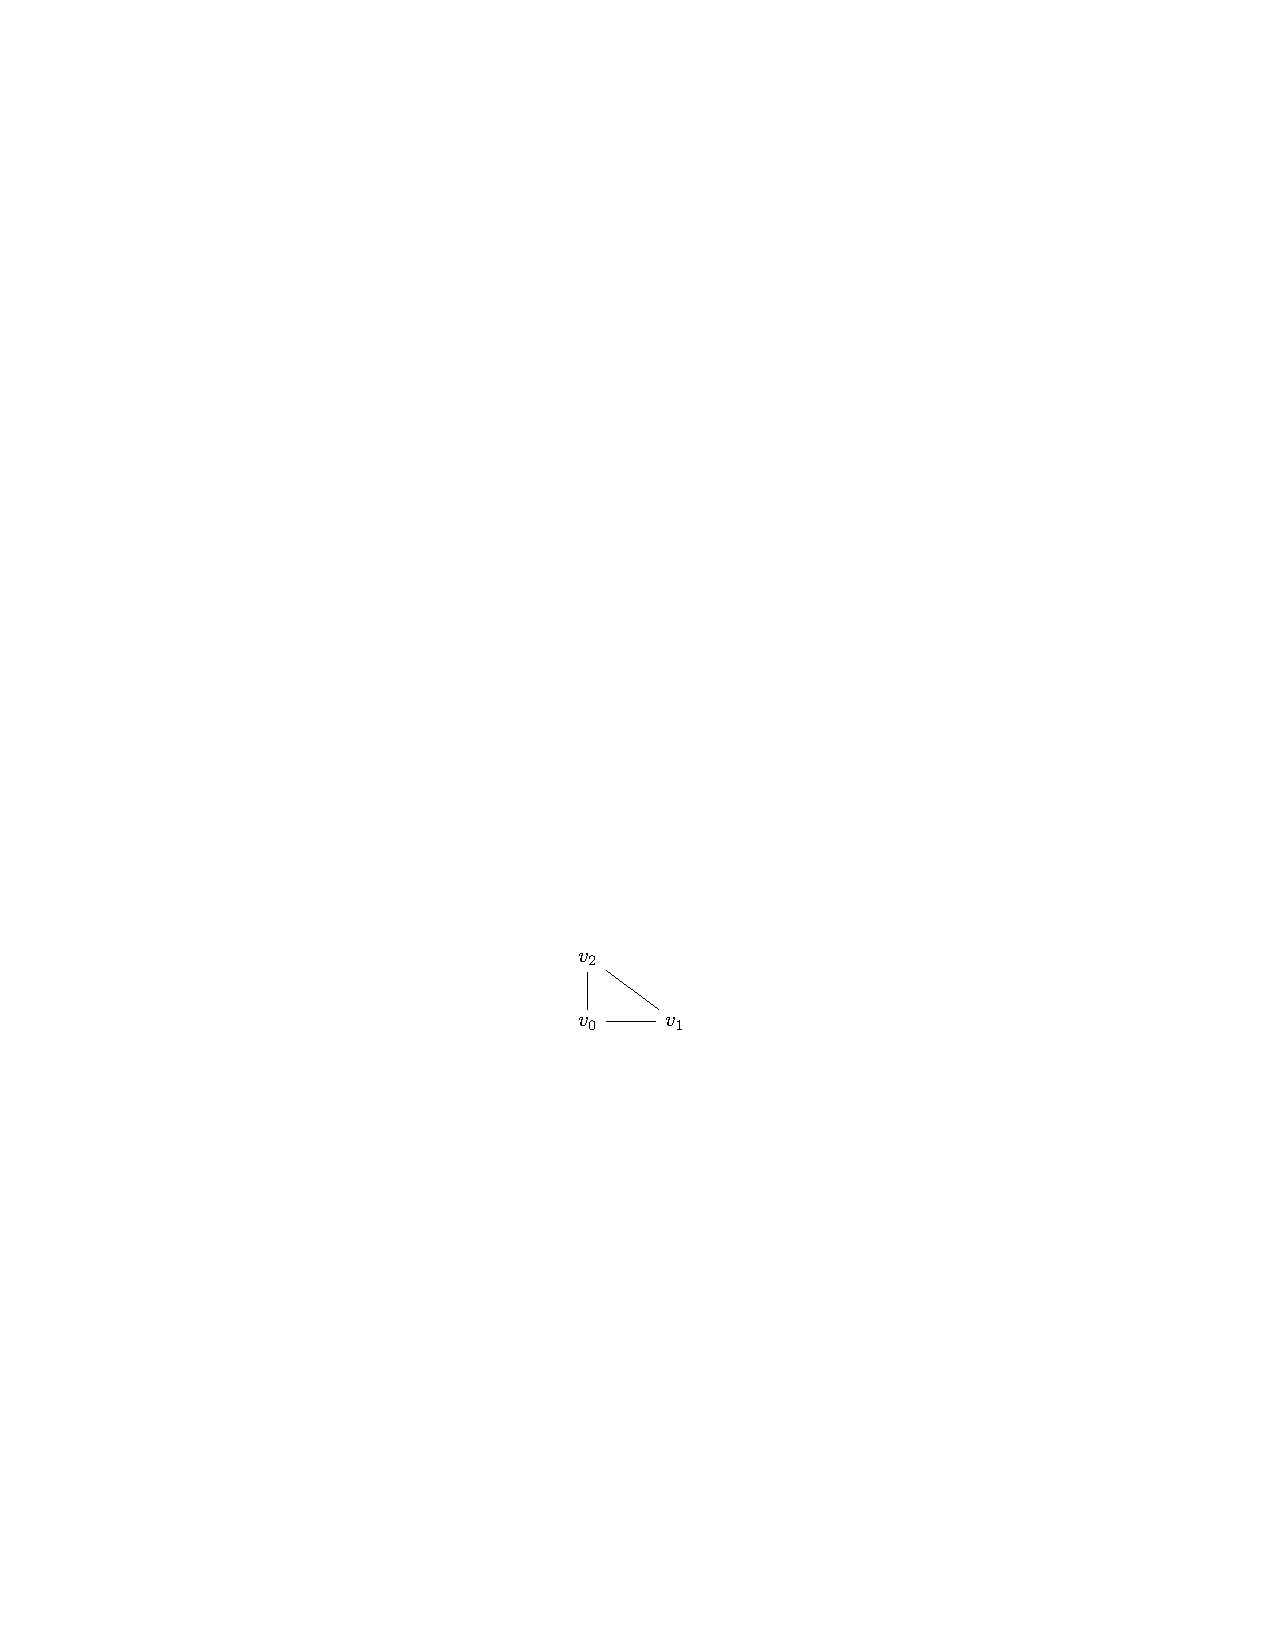
\includegraphics[width=0.1364\linewidth]{images/diagram-4-100.pdf}}}.}
每个顶点 $v_i$ 对应一个锥 $\tau_i$。它们正好是图~\ref{fig:4.1} 中的三个锥，因此 $\Sigma_\Xi$ 如图~\ref{fig:4.6} 所示。
\end{example}
\begin{Note}{4.12}把 $\Xi$ 按正比例缩放，或对它的各个面作保持组合类型的小幅平行移动，均不改变法扇。\end{Note}
\thmnum{definition}{15}\begin{definition}\label{def:4.15}
与 $\Xi$ 关联的环面簇定义为 $X(\Sigma_\Xi)$。
\end{definition}
\examnum{25}\begin{example}\label{ex:4.25}
若
\Eq{4.101}{\Xi=\conv\{0,e_1,\ldots,e_d\},}
则 $X(\Sigma_\Xi)\simeq\PP^d$。当 $d=2$ 时，除去缩放与平移，这就是例题~\ref{ex:4.24}：取 $(0,0),(0,1),(1,0)$ 的凸包，可得到例题~\ref{ex:4.10} 中的 $\PP^2$。当 $d=3$ 时，相应多胞体是四面体。
\end{example}
\SourcePage{77}
\OriginalFigure{fig-4-7.pdf}{0.5202}{在此图上方取锥得到一个扇，它有7个极大锥。}{fig:4.7}
\examnum{26}\begin{example}\label{ex:4.26}
回忆 Hirzebruch 曲面 $X=\PP(\OO_{\PP^1}\oplus\OO_{\PP^1}(a))$，其中 $a\ge0$。它由 $X(\Sigma_\Xi)$ 给出，$\Xi$ 为如下梯形：
\Eq{4.102}{\vcenter{\hbox{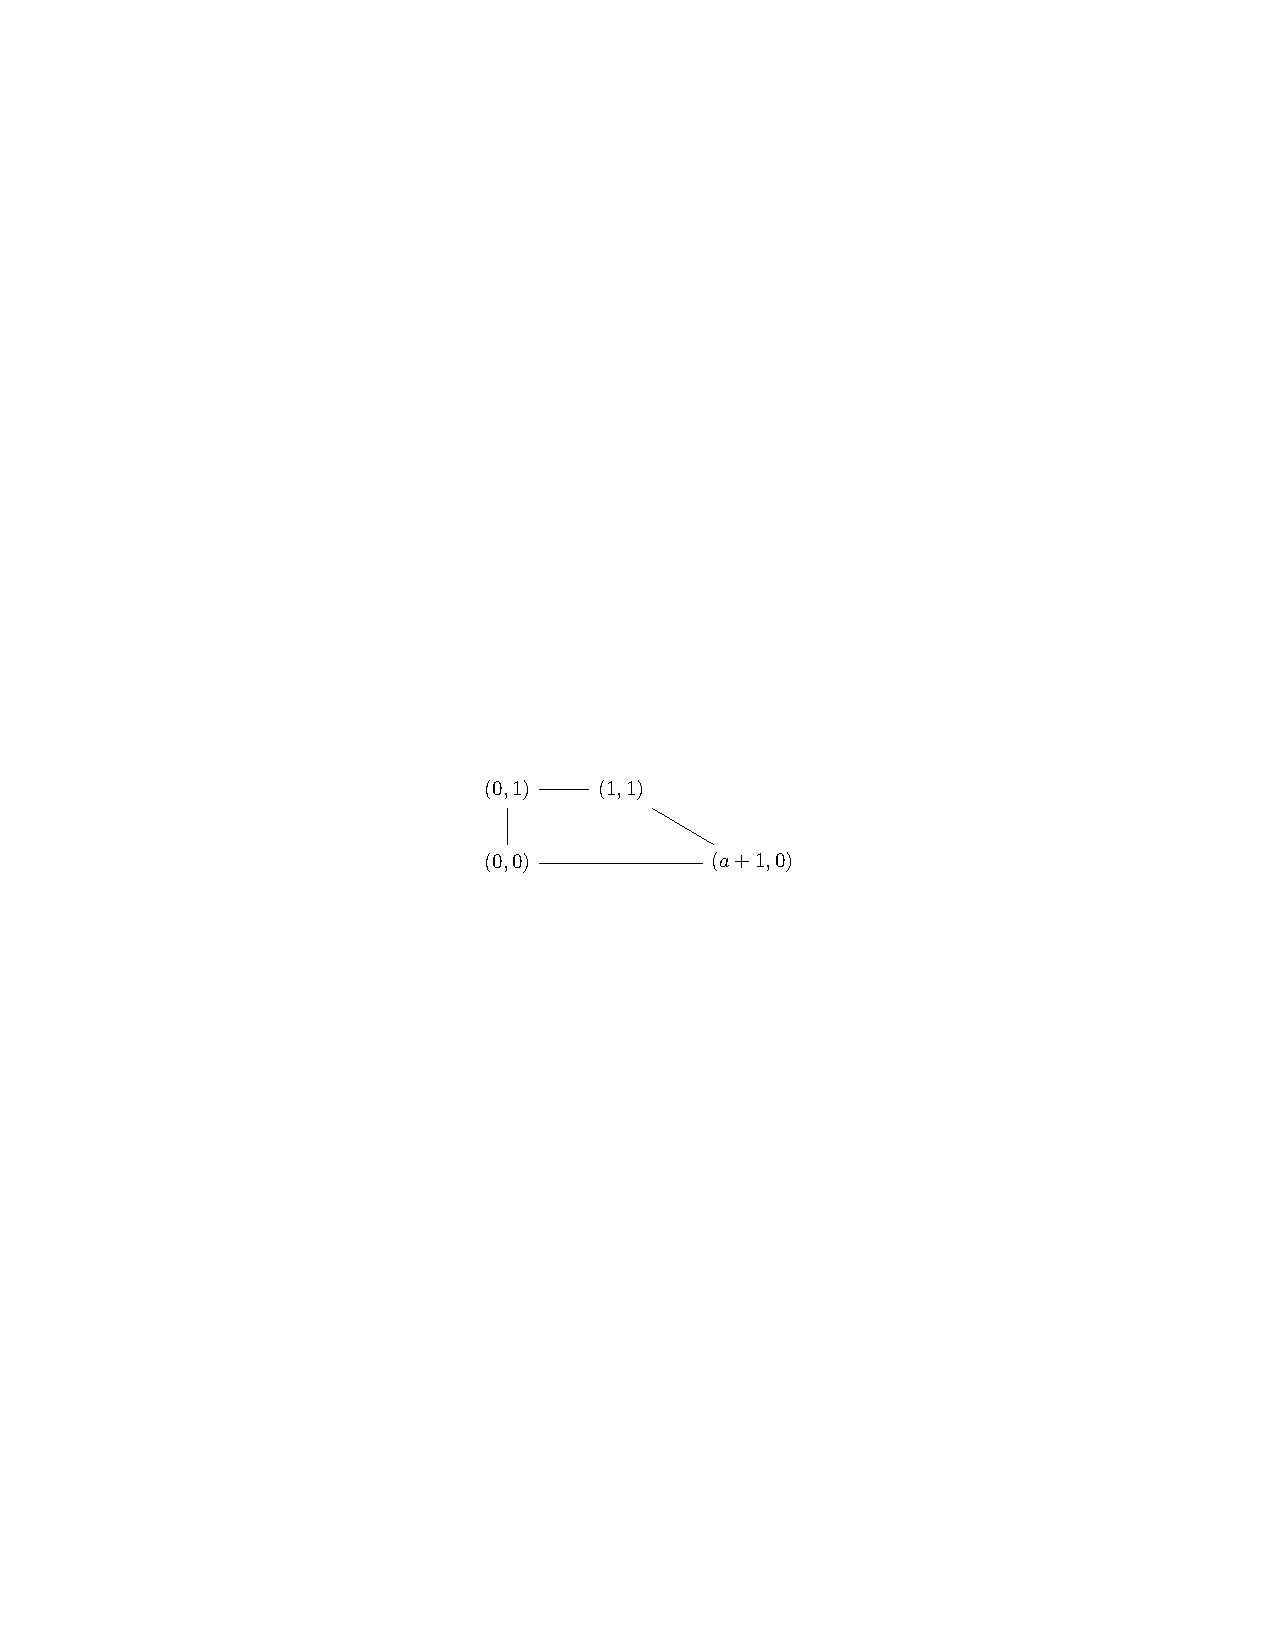
\includegraphics[width=0.3847\linewidth]{images/diagram-4-102.pdf}}}.}
\end{example}
\Lecture{21}{2019年11月7日}
\thmnum{proposition}{13}\begin{proposition}\label{prop:4.13}
$\operatorname{Proj}k[C(\Xi)\cap(M\oplus\ZZ)]\simeq X(\Sigma_\Xi)$。
\end{proposition}
\begin{proof}
一旦理解这个 $\operatorname{Proj}$ 的构造，结论便是同义反复。具体地，在单项式 $\chi^{(v,1)}$ 处作去齐次化，会得到形如 $\Spec k[\sigma^\vee\cap M]$ 的开集，于是结论成立。
\end{proof}
\begin{Note}{4.13}有如下典范双射：
\Eq{4.103}{\left\{\text{满维有理多面体 }\Xi\subset M_{\RR}\right\}\simeq\left\{(\Sigma,\varphi):\begin{array}{l}\Sigma\text{ 是 }N_{\RR}\text{ 中支撑凸的扇},\\\varphi:|\Sigma|\to\RR\text{ 是有理、严格凸的分段线性函数}\end{array}\right\}.}
特别地，左侧的顶点 $v_i$ 对应右侧的极大锥 $\sigma$，且 $\varphi|_\sigma=v_i:N_{\RR}\to\RR$。反向映射把 $\varphi$ 送到 $(\Sigma,\varphi)$ 的 Newton 多面体，记为 $\Xi(\Sigma,\varphi)$。$\Xi\mapsto\Xi+m$ 对应于 $(\Sigma,\varphi)\mapsto(\Sigma,\varphi+m)$。
\end{Note}
\begin{Note}{4.14}并非每个扇都能这样得到。二维时每个有限扇都可以支持相应的严格凸分段线性函数；三维及更高维则不然。\end{Note}
\begin{Counterexample}{2}\label{counterex:2}
在图~\ref{fig:4.7} 上方取锥。所得扇不能支持严格凸的分段线性函数；等价地，该三角剖分不是“正则”的。
\end{Counterexample}
\examnum{27}\begin{example}\label{ex:4.27}
回忆例题~\ref{ex:4.21}，其上方的锥为
\Eq{4.104}{C(\Xi)=\langle(1,0,0),(0,1,0),(1,0,1),(0,1,1)\rangle.}
\SourcePage{78}
于是
\Eq{4.105}{k[C(\Xi)\cap(M\oplus\ZZ)]\simeq k[x,y][U,V]/(xV-yU).}
取 $\operatorname{Proj}$，得到吹起
\Eq{4.106}{\operatorname{Proj}k[C(\Xi)\cap(M\oplus\ZZ)]\simeq\operatorname{Bl}_0\mathbb A^2.}
从扇的角度看，先取给出 $\mathbb A^2$ 的右上象限，再把它细分为由 $(1,0),(1,1)$ 生成的锥，以及由 $(1,1),(0,1)$ 生成的锥。关键在于，截去多面体的角对应于其法扇 $\Sigma_\Xi$ 的射影细分。\footnote{即细分支持一个严格凸的分段线性函数。}
\end{example}
\section{环面簇上的 Weil 除子}
设 $X$ 为 $d$ 维环面簇，扇为 $\Sigma$，射线为 $\RR_{\ge0}v_1,\ldots,\RR_{\ge0}v_r$，各 $v_i$ 均为本原向量。每个 $v_i$ 给出一个 $d-1$ 维环面分层，即 Weil 除子 $D_i$，称为环面素除子。记
\Eq{4.107}{\operatorname{Div}^T X\subset\operatorname{Div}X}
为 $T$ 不变 Weil 除子的子群。注意，
\Eq{4.108}{\operatorname{Div}^T X=\bigoplus_{i=1}^r\ZZ[D_i].}
\Term{chuzileiqun}{除子类群}为
\Eq{4.109}{\operatorname{Cl}X=A_{d-1}(X)=\operatorname{Div}X/{\sim_{\text{有理等价}}}.}
\thmnum{proposition}{14}\begin{proposition}\label{prop:4.14}
以下序列正合：
\Eq{4.110}{0\longrightarrow M/(M\cap|\Sigma|^\perp)\xrightarrow{m\mapsto\operatorname{div}(\chi^m)}\operatorname{Div}^T X\longrightarrow\operatorname{Cl}X\longrightarrow0,}
其中
\Eq{4.111}{\operatorname{div}(\chi^m)=\sum_{i=1}^r\operatorname{ord}_{D_i}(\chi^m)D_i.}
\end{proposition}
\begin{proof}
$k[M]$ 是唯一分解整环，因而
\Eq{4.112}{0=\operatorname{Cl}\Spec k[M]=\operatorname{Cl}T=\operatorname{Cl}(X\setminus D).}
由此 $A_{d-1}(D)=\operatorname{Div}^T(X)\twoheadrightarrow\operatorname{Cl}X$。
若 $\sum n_iD_i$ 在此映射的核中，则存在 $f\in k(X)^\times$，使 $\operatorname{div}(f)=\sum n_iD_i$。这意味着
\Eq{4.113}{f|_{X\setminus D}\in k[M]^\times=k^\times\times M,}
即 $f=\lambda\chi^m$，其中 $\lambda\in k^\times$、$m\in M$。不妨令 $\lambda=1$。
\end{proof}
\SourcePage{79}
注意 $\operatorname{ord}_{D_i}\chi^m=\langle v_i,m\rangle$。为说明这一点，选取 $N$ 的格基，令第一个基向量为 $e_1=v_i$，其余基向量任意补齐。记对偶基为 $e_j^*$，则 $D_i$ 中的稠密环面为
\Eq{4.114}{T_{D_i}=\Spec k[\chi^{\pm e_2^*},\ldots,\chi^{\pm e_d^*}],}
它位于开集
\Eq{4.115}{X\supset U_i=\Spec k[\chi^{e_1^*},\chi^{\pm e_2^*},\ldots,\chi^{\pm e_d^*}].}
写 $m=\sum_jm_je_j^*$，则 $\chi^m=\prod_j(\chi^{e_j^*})^{m_j}$，因此
\Eq{4.116}{\operatorname{ord}_{D_i}\chi^m=m_1=\langle m,v_i\rangle.}
\section{\texorpdfstring{$\operatorname{Cl}(\PP^n)$}{Cl(Pⁿ)}}
\thmnum{corollary}{15}\begin{corollary}\label{cor:4.15}
$\operatorname{Cl}(\PP^n)=A_{n-1}(\PP^n)=\ZZ H$，其中 $H$ 是一个超平面。次数映射 $\operatorname{Cl}(\PP^n)\to\ZZ$ 由与直线相交给出。
\end{corollary}
\begin{proof}
有短正合序列
\Eq{4.117}{0\longrightarrow\ZZ^n\xrightarrow{m\mapsto(\langle v_i,m\rangle)_i}\ZZ^{n+1}\xrightarrow{(a_i)\mapsto\sum_i a_i}\ZZ\longrightarrow0,}
而相应射线为
\Eq{4.118}{\Sigma_{\PP^n}[1]=\{\RR_{\ge0}e_1,\ldots,\RR_{\ge0}e_n,\RR_{\ge0}(-e_1-\cdots-e_n)\}.}
\end{proof}
\section{环面簇上的 Cartier 除子}
回忆，Cartier 除子群为
\Eq{4.119}{\operatorname{CaDiv}X=\Gamma(X,\mathcal K^\times/\OO_X^\times),}
其中 $\mathcal K$ 为全商环层。若 $X$ 整，则 $\mathcal K$ 是茎为函数域 $K(X)$ 的常值层。于是 Cartier 除子可由数据
\Eq{4.120}{\{(U_i,f_i):f_i\in K(X)^\times,\ f_i/f_j\in\OO_X^\times(U_i\cap U_j)\text{ 对所有 }i,j\}}
表示，并有 $\operatorname{CaDiv}X\hookrightarrow\operatorname{Div}X$。
\thmnum{lemma}{16}\begin{lemma}\label{lem:4.16}
设 $X=\Spec k[\sigma^\vee\cap M]$ 为仿射环面簇。$T$ 不变 Weil 除子 $D$ 是 Cartier 除子，当且仅当存在 $m\in M$ 使 $D=\operatorname{div}(\chi^m)$。
\end{lemma}
\thmnum{proposition}{17}\begin{proposition}\label{prop:4.17}
设 $\Sigma$ 为 $N_{\RR}$ 中的扇，相应环面簇为 $X_\Sigma$。则
\Eq{4.121}{\operatorname{CaDiv}^T(X_\Sigma)\simeq\mathrm{PL}(\Sigma)=\{\varphi:|\Sigma|\to\RR:\varphi\text{ 在每个锥上由 }M\text{ 中的线性函数给出}\}.}
此对应把 $\varphi$ 映为 $\sum_i\varphi(v_i)D_i$，其中 $v_i$ 为射线的本原生成向量，射线写成 $\RR_{\ge0}v_i$。
\end{proposition}
\section{Picard 群}
\thmnum{proposition}{18}\begin{proposition}\label{prop:4.18}
$\Pic(X_\Sigma)=\mathrm{PL}(\Sigma)/M=\operatorname{CaCl}X$，其中 $\operatorname{CaCl}X=\operatorname{CaDiv}(X)/{\sim_{\text{有理等价}}}$ 是 Cartier 除子类群。
\end{proposition}
\thmnum{corollary}{19}\begin{corollary}\label{cor:4.19}
$\Pic(X_\Sigma)$ 是离散的。若 $\Sigma$ 含有满维锥，则它无挠；此时，对 $\varphi\in\mathrm{PL}(\Sigma)$，若 $\varphi$ 是由 $M_{\RR}$ 中一个向量给出的全局线性函数，则它实际上来自 $M$。
\end{corollary}
\Lecture{22}{2019年11月12日}
\SourcePage{80}
\section{丰环面除子}
\thmnum{proposition}{20}\begin{proposition}\label{prop:4.20}
设有限扇 $\Sigma$ 的支撑凸，极大锥均满维，$\varphi\in\mathrm{PL}(\Sigma)$，并令 $D=\sum_i\varphi(v_i)D_i$ 为相应 Cartier 除子。则 $\OO_X(D)$ 丰当且仅当 $\varphi$ 严格凸。
\end{proposition}
\begin{proof}
$\Leftarrow$：令 $\Xi$ 为 Newton 多面体，有
\Eq{4.122}{X=X(\Sigma_\Xi)\simeq\operatorname{Proj}k[C(\Xi)\cap(M\oplus\ZZ)].}
而 $\OO_X(D)$ 对应于 $\OO_X(1)$，因此丰，事实上甚丰。

$\Rightarrow$：令 $\rho\in\Sigma[d-1]$ 为不在 $\partial|\Sigma|$ 中的余维一锥。$\varphi$ 沿 $\rho$ 的“折角”记为 $K_\rho(\varphi)\in\ZZ$。写 $\rho=\sigma_1\cap\sigma_2$，其中 $\sigma_i$ 为极大锥，且
\Eq{4.123}{\varphi|_{\sigma_1}=m_1\in M,\qquad\varphi|_{\sigma_2}=m_2\in M.}
记 $\check d_\rho\in M$ 为秩一格 $\rho^\perp\cap M$ 的唯一满足 $\check d_\rho|_{\sigma_2}\ge0$ 的本原生成元。则 $m_2-m_1=K_\rho(\varphi)\check d_\rho\in\rho^\perp$。
\begin{custom}{事实 7}\hypertarget{fact:7}{}$\varphi$ 严格凸当且仅当对每个这样的 $\rho$，都有 $K_\rho(\varphi)>0$。\end{custom}
\begin{custom}{事实 8}\hypertarget{fact:8}{}$K_\rho(\varphi)=\deg\bigl(\OO_X(D)|_{X(\Sigma_\rho)}\bigr)$。\end{custom}
若 $D$ 丰，则这个次数为正。
\end{proof}
